\chapter{Credit Derivatives}

A credit derivative is a financial contract that allows parties to minimize their exposure to credit risk. Credit derivatives consist of a privately held, negotiable bilateral contract traded over-the-counter (OTC) between two parties in a creditor/debtor relationship. These allow the creditor to effectively transfer some or all of the risk of a debtor defaulting to a third party. This third party accepts the risk in return for payment, known as the premium.

Credit default swaps have been already introduced in Chapter~\ref{sec:credit-default-swaps}, here two more kind of credit derivatives will be presented: Basket Default Swaps and Collateralized Debt Obligations (CDO).

\section{Basket Default Swaps}
\label{basket-default-swaps}

A Basket Default Swaps (BDS) is a credit derivative on a portfolio of reference entities.

This kind of contracts are very similar to normal CDS except for the protection they offer. With respect to a basket of reference entities, a first-to-default BDS provides insurance for only the first default, a second-to-default BDS provides insurance for only the second default, or a nth-to-default BDS provides insurance for only the $n^{th}$ default. 

For example, in the latter, the seller does not make any payment to the protection buyer for the first $n-1$ defaulted entities, and makes it only for the $n^{th}$. Once there has been this payment the swap terminates.

The cost of protection in nth-to-default basket is obviously dependent on default correlations. Suppose that a basket of 100 reference entities is used to define a 5-year nth-to-default swap and that each reference entity has a 2\% probability of defaulting during the next 5 years. When the default correlation between the reference entities is zero (i.e. they are uncorrelated), the binomial distribution (see Appendix~\ref{binomial-distribution}) shows that the probability of one or more defaults during 5 years is 86.74\% and the probability of ten or more defaults is 0.0034\%.

\begin{ipython}
from scipy.stats import binom

b = binom(100, 0.02)
print(f"P(>=1) : {1 - b.cdf(0)}")
print(f"P(>=10): {1 - b.cdf(9)}")
\end{ipython}
\begin{ioutput}
P(>=1) : 0.8673804441052471
P(>=10): 3.441680604299169e-05
\end{ioutput}

A first-to-default is therefore quite valuable whereas a tenth-to-default swap is worth almost nothing.

As the default correlation increases the probability of one or more defaults declines but that for ten or more defaults increases too. In the limit where default correlations are perfect the probability of one or more defaults equals the probability of ten or more and it is 2\%. This is because in this extreme situation the reference entities are essentially the same: either they all default (with 2\% probability) or none of them default (with 98\% probability). Similarly for the value of the basket default swaps.

We now present some numerical results for a nth-to-default basket with two complementary approaches. We assume that principals and expected recovery rates are the same for all underlying reference assets. 

The valuation procedure is similar to that for a regular CDS. There it was based on the probability that a default occurred between times $t_1$ and $t_2$, see Section~\ref{sec:cds_valuation}. Here instead it will rely on the probability that the $n^{th}$ default happened between times $t_1$ and $t_2$. The buyer of protection makes quarterly payments at a specified rate until the $n^{th}$ default occurs, in which case the seller pays $F\cdot(1-R)$, or the end life of the contract is reached. 

Two complementary approaches are going to be presented, each with different ways to compute the default probabilities to construct the needed credit curve.

\subsection{Basket Default Swaps Valuation (Monte Carlo)}
\label{basket-cds-valuation-with-monte-carlo}

\begin{finmarkets}
In the following we develop a \texttt{BasketDefaultSwaps} class that is able to valuate the basket NPV using a Monte Carlo approach relying on a numerical multivariate Gaussian copula. 
The logic of the class relies on computing the contract NPV of the contract using a provided discount curve and the appropriate credit curve determined as described above.
\end{finmarkets}

\begin{ipython}
import numpy as np
from finmarkets import CreditCurve, CreditDefaultSwap

class BasketDefaultSwaps:
    def __init__(self, nominal, N, start_date, maturity, spread, 
                 tenor="3m", recovery=0.4):
        self.cds = CreditDefaultSwap(nominal, start_date, maturity,
                                     spread, tenor, recovery)
        self.N = N
        self.cc = None

    def credit_curve(self, n_defaults, copula_func, default_prob, obs_date, 
                     pillars, simulations=100000):
        copula_sample = copula_func.sample(simulations)
        default_times = default_prob.ppf(copula_sample)

        Ts = [(p-obs_date).days/365 for p in pillars]
        ndps = []
        for t in Ts:
            entity_defs_per_sim = np.sum(default_times <= t, axis=1)
            tot_defs = np.sum(entity_defs_per_sim >= n_defaults)
            ndps.append(1 - tot_defs/simulations)
        self.cc = CreditCurve(obs_date, pillars, ndps)

    def npv(self, dc):
        if self.cc is None:
            print ("Need to call credit_curve method first !")
            return None
        return self.cds.npv(dc, self.cc)

    def breakeven(self, dc):
        if self.cc is None:
            print ("Need to call credit_curve method first !")
            return None
        return self.cds.breakevenRate(dc, self.cc)
\end{ipython}

Consider a 2-years 3rd-to-default basket of 10 reference entities, with a spread of 1\%, in the situation where the Gaussian copula correlation varies between is 0.3, the expected recovery rate, $R$, is $40\%$, and the term structure of interest rates is assumed to be flat at 5\%. The default probabilities $Q(t)$ for the ten entities are generated by Poisson processes, see Sec.~\ref{sec:poisson_process}, with constant default intensities, $\lambda_i=0.06$, such that $Q(t) = 1 - e^{-\lambda t}$

\begin{ipython}
import numpy as np
from finmarkets import DiscountCurve, CreditCurve, PossionProcess
from scipy.stats import multivariate_normal, norm
from datetime import date
from dateutil.relativedelta import relativedelta

n_cds = 10
rho = 0.3
cov = np.ones(shape=(n_cds, n_cds))*rho
np.fill_diagonal(cov, 1)
copula = GaussianCopula(n_cds, cov)
poisson = PoissonProcess(l=0.06)

obs_date = date.today()
start_date = obs_date
pillar_dates = [obs_date + relativedelta(years=i) for i in range(6)]
dfs = [1/(1+0.05)**i for i in range(1, 6)]
dc = DiscountCurve(obs_date, pillar_dates, dfs)

np.random.seed(1)
basket = BasketDefaultSwaps(1, n_cds, start_date, "2y", 0.01)
basket.credit_curve(n_defaults=3, copula_func=copula, default_prob=poisson, 
                    obs_date=obs_date, pillars=pillar_dates)
print (f"NPV: {basket.npv(dc):3f} EUR")
\end{ipython}
\begin{ipython}
NPV: 0.0708 EUR
\end{ipython}

Using the \texttt{BasketDefaultSwaps} class it is possible to check how the value (and the spread) of such BDS varies as a function of the correlation $\rho$ and the number of defaults (\texttt{n\_defaults}).

Figures~\ref{fig:bds_value_mc} show the resulting distributions. A 1st-to-default is quite valuable for independent defaults, then as correlation increases its value decreases down to the minimum for $\rho=1$.
Other BDS with higher number of required defaults, are less valuable when the default probability is low but increase with correlation. Anyway all of them reach the asymptotic value for $\rho=1$ where all the reference assets act as a single name and can only default all together.

Notice the jiggling nature of each curve in Fig.~\ref{fig:bds_value_mc} (left) this is due to the fluctuation in the results due to Monte Carlo approximation (i.e. finite sampling).

\begin{figure}[htb]
\centering
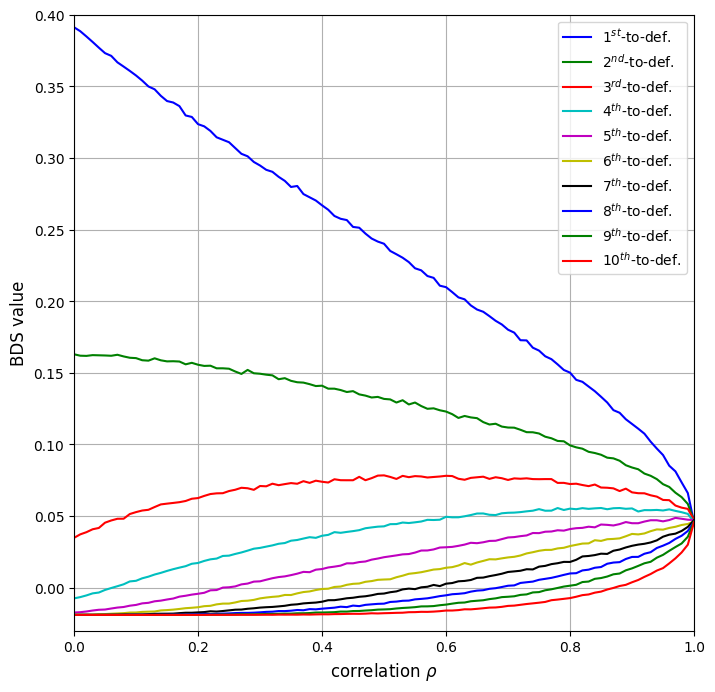
\includegraphics[width=0.45\textwidth]{figures/bds_value_mc}
\quad
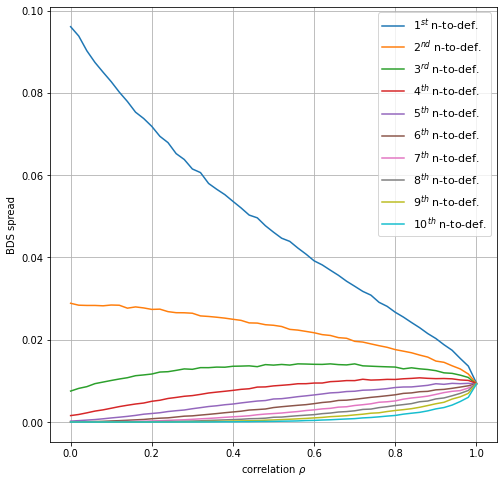
\includegraphics[width=0.45\textwidth]{figures/bds_spread_mc}
\caption{BDS value (left) and spread (right) as a function of the default correlation $\rho$ and the number of required defaults, using Monte Carlo simulation to determine the credit curve.}
\label{fig:bds_value_mc}
\end{figure}

\subsection{Basket Default Swap Valuation (One Factor Copula Model)}
\label{basket-cds-valuation-under-market-standard-model}

In this case, since we are under the assumption of the One Factor Copula model, the strategy is:
\begin{itemize}
\item compute the correlated default probability of each name according to 
\begin{equation}
Q^{\textrm{corr}}(t|M) = \Phi\left(\cfrac{\Phi^{-1}[Q(t)]-\sqrt{\rho} M}{\sqrt{1-\rho}}\right)
\end{equation}
\item calculate the probability of having at least $j$ defaults using the binomial distribution
\begin{equation}
P_{\mathrm{def}}(l(t|m) \ge j) = \sum_{k=j}^{N}\left[  \cfrac{N!}{k!(N-k)!}Q^{\textrm{corr}}(t|M)^k(1-Q^{\textrm{corr}}(t|M))^{N-k}\right]
\end{equation}
\item create a \textbf{credit curve}, $CC(P_{\mathrm{def}})$ according to those probabilities;
\item re-use the \texttt{CreditDefaultSwap} class to compute NPV and break-even rate with a discount curve $DC$ and the appropriate credit curve determined above, through integration of
\begin{equation}
\mathrm{NPV}_{BDS}(DC, CC(P_{\mathrm{def}})) = \int_{-\infty}^{\infty}{\mathrm{NPV}_{CDS}(DC, CC(P_{\mathrm{def}})|M) f_M(m)dm} 
\end{equation}
\end{itemize}

To perform the integrals needed by the basket default swap valuation it can be used the method described in Section~\ref{sec:integration}.

\begin{ipython}
from finmarkets import CreditCurve, CreditDefaultSwap
from scipy.stats import norm, binom
from scipy.integrate import quad
import numpy as np

class BasketDefaultSwapsOneFactor:
    def __init__(self, nominal, N, rho, start_date, maturity,
                 spread, tenor="3m", recovery=0.4):
        self.N = N
        self.rho = rho
        self.cds = CreditDefaultSwap(nominal, start_date, maturity,
                                     spread, tenor, recovery)

    def one_factor_model(self, M, f, obs_date,
                         Q_dates, Q, dc, ndefaults):
        P = norm.cdf((norm.ppf(Q) - np.sqrt(self.rho)*M)/np.sqrt(1-self.rho))
        b = binom(self.N, P)
        S = 1 - (1 - b.cdf(ndefaults-1))
        cc = CreditCurve(obs_date, Q_dates, S)
        return f(dc, cc)*norm.pdf(M)
            
    def breakeven(self, obs_date, Q_dates, Q, dc, ndefaults):
        s = quad(self.one_factor_model, -np.inf, np.inf, 
                 args=(self.cds.breakevenRate, Q_dates, Q, dc, ndefaults))
        return s[0]
    
    def npv(self, obs_date, Q_dates, Q, dc, ndefaults):
        s = quad(self.one_factor_model, -np.inf, np.inf, 
                 args=(self.cds.npv, Q_dates, Q, dc, ndefaults))
        return s[0]
\end{ipython}

Let's repeat a similar scan of the BDS value as a function of the correlation $\rho$ and the number of defaults as performed above. The parameters of the BDS remain unchanged.

\begin{ipython}
from finmarkets import DiscountCurve
from datetime import date
from dateutil.relativedelta import relativedelta
import numpy as np

n_cds = 10
l = 0.06
rho = 0.3

obs_date_date = date.today()
start_date = obs_date
pillar_dates = [obs_date + relativedelta(years=i) for i in range(6)]
dfs = [1/(1+0.05)**i for i in range(1, 6)]
dc = DiscountCurve(obs_date, pillar_dates, dfs)
Q = [1-np.exp(-(l*t)) for t in range(1, 6)]

basket = BasketDefaultSwapsOneFactor(1, n_cds, rho, obs_date, 0.01, "2y")
print(basket.npv(pillar_dates, Q, dc, 3))
\end{ipython}
\begin{ioutput}
0.01791086281290842
\end{ioutput}

\begin{figure}[htb]
\centering
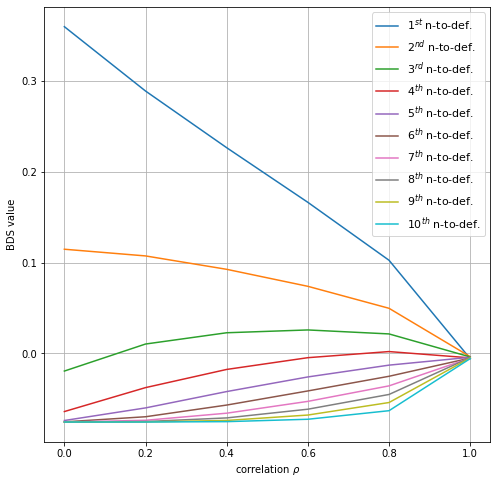
\includegraphics[width=0.5\textwidth]{figures/bds_value_one_factor}
\caption{BDS value as a function the default correlation $\rho$ and the number of required defaults, under One Factor Gaussian Copula.}
\label{fig:bds_value_one_factor}
\end{figure}

Figure~\ref{fig:bds_value_one_factor} shows that the results are close to what obtained with the previous model. It has to be noticed though that the integration performed here is much slower than the simulation with Monte Carlo sampling.

\section{Collateralized Debt Obligation}\label{collateralized-debt-obligation}

A Collateralized Debt Obligation (CDO) is a credit derivative where the issuer gather risky assets and repackage them into discrete classes, called \emph{tranches}, which are defined on the level of credit risk assumed by the investor. These tranches of securities become the final investment product.

Tranches are named to reflect their risk profile: \emph{senior}, \emph{mezzanine} and \emph{subordinated/equity} and are delimited by an attachment ($L$) and a detachment point ($U$), which represent the percentages of the \textbf{total} principal defining their boundaries. For example, a 5-10\% tranche has an attachment point of 5\% and a detachment point of 10\%. 

Each of these tranches has a different level of seniority relative to the others in the sense that a senior tranche has coupon and principal payment priority over a mezzanine, while a mezzanine tranche has coupon and principal payment priority over an equity one. 

Indeed they receive returns using a set of rules known as \emph{waterfall}. Incomes of the portfolio are first used to provide returns to the most senior tranche, then to the next and so on. So senior tranches are generally safest because they have the first claim on the collateral, although they'll offer lower coupon rates.

It is important to note that a CDO only redistributes the total risk associated with the underlying pool of assets to the priority ordered tranches; it neither reduces nor increases the total risk associated with the pool.

There are various kind of CDOs:
\begin{itemize}
\item in a \textbf{Cash CDO} the reference portfolio consists of corporate bonds owned by the CDO issuer. Cash flows from collateral are used to pay principal and interests to investors. If such cash flows prove inadequate, rewards are paid to tranches according to their seniority. Figure~\ref{fig:cdo_structure} shows a typical structure of a Cash CDO;

\begin{figure}[htb]
\centering
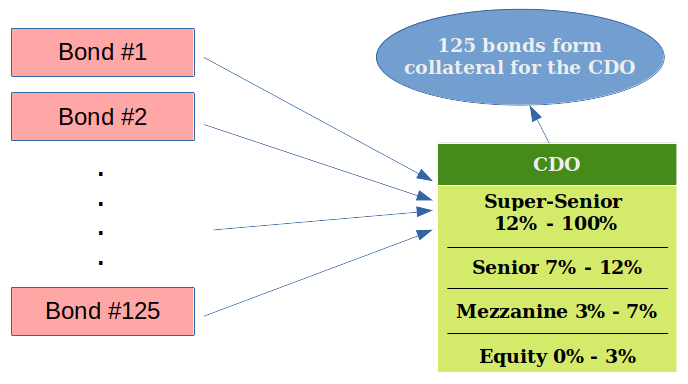
\includegraphics[width=0.7\textwidth]{figures/cdo_structure}
\caption{Typical structure of a Cash CDO, with the reference portfolio made of bonds, which form the contract collateral.}
\label{fig:cdo_structure}
\end{figure}

\item in a \textbf{Synthetic CDO} the underlying reference portfolio is no longer "physical" (e.g. portfolio of bonds or loans), instead it is a \emph{fictitious} portfolio consisting of a number of reference obligations each with an associated notional amount. The value of a synthetic CDO usually comes from insurance premiums of credit default swaps paid for by investors. The investment logic is that sellers assume the underlying assets will perform while investors that will sooner or later default.
\end{itemize}

\subsection{Cash CDO Expected Losses}
\label{sec:expected_losses}

Consider a Cash CDO made of 125 bonds with a maturity of 1 year. Each bond pays a coupon of one unit after 1 year and it has not yet defaulted (the recovery rate $R$ is assumed to be 0). We are interested in the following three tranches: equity ([0, 3] defaults), mezzanine ([4, 6] defaults) and senior ([7, 9] defaults), see Fig.~\ref{fig:cdo_ex_1} (note that in this particular case tranches are identified through the number of defaults and not with principal percentages). 

\begin{figure}[htb]
	\centering
	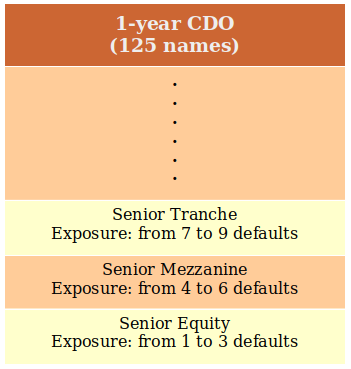
\includegraphics[width=0.5\textwidth]{figures/ex_cdo_1}
	\caption{Structure of the simple Cash CDO considered in the example.}
	\label{fig:cdo_ex_1}
\end{figure}

Assume also that one year default probabilities are identical for each bond ($Q$) and that the correlation between each pair is also identical and equal to $\rho$. Under these assumptions we are in the position to use the Gaussian Copula Model. 

We are interested in the expected losses for each tranche as a function of the correlation $\rho$.

The probability of having $l$ defaults, conditional to the market parameter $M$ will follow a binomial distribution given by
\begin{equation}
p(l|M) = \binom{N}{l}\mathcal{Q}_M^l (1-\mathcal{Q}_M)^{N-l}
\label{eq:def_prob_ex_cdo_1}
\end{equation}
where $N$ is the number of bonds in the portfolio and 
\begin{equation}
\mathcal{Q}_M = \Phi\left(\cfrac{\Phi^{-1}(Q)-\sqrt{\rho}M}{\sqrt{\-\rho}}\right)
\end{equation}
where $\Phi$ is the standard normal CDF and $Q$ the marginal probability of default within 1 year of a single name.

From the definition of each tranche with have that the expected losses are
\begin{itemize}
	\item $\mathbb{E}_{\textrm{equity loss}}(l, \mathcal{Q}_M)=3\cdot p(l\ge 3|M) + \sum_{k=1}^{2}k\cdot p(l=k|M)$
	\item $\mathbb{E}_{\textrm{mezzanine loss}}(l, \mathcal{Q}_M)=3\cdot p(l\ge 6|M) + \sum_{k=1}^{2}k\cdot p(l=k+3|M)$
	\item $\mathbb{E}_{\textrm{senior loss}}(l, \mathcal{Q}_M)=3\cdot p(l\ge 9|M) + \sum_{k=1}^{2}k\cdot p(l=k+6|M)$
\end{itemize}
	
Each probability can be calculated by integrating the above with respect to $M$
	
\begin{equation} 
\mathbb{E}_{\mathrm{tranche}} = \int_{-\infty}^{\infty}{\mathbb{E}_{\mathrm{tranche}}(l, \mathcal{Q}_M) f_M(m)dm}
\end{equation}

Let's see the corresponding \texttt{python} implementation: first we import the necessary modules and define the needed constants.

\begin{ipython}
from scipy.stats import binom, norm
from scipy.integrate import quad
import numpy as np

N = 125
C = 1
R = 0
q = 0.02
tranches = [[1,3],[4, 6],[7,9]]
\end{ipython}

Then we define a function \texttt{p} which implements the expected losses for each tranche according to Eq.~\ref{eq:def_prob_ex_cdo_1}.
The function depends on the parameter \texttt{M}, and takes as inputs the correlation \texttt{rho} and the tranche attach-detach limits.
	
\begin{ipython}
def p(M, rho, lims):
    qM = norm.cdf((norm.ppf(q)-np.sqrt(rho)*M)/(np.sqrt(1-rho)))
    pN = binom(N, qM)
    loss = 3*(pN.cdf(N) - pN.cdf(lims[1]-1))
    for i in range(lims[0], lims[1]):
        index = i-lims[0]+1
        loss += index*pN.pmf(i)
    return norm.pdf(M)*loss
\end{ipython}

Finally we loop over a range of possible values for the correlation on each tranche to draw the plot of the expected losses vs correlation, shown in Fig.~\ref{fig:losses_rho}.

\begin{ipython}
res = [[],[],[]]
for i in range(len(tranches)):
    for rho in np.arange(0, 1.05, 0.05):
        if rho == 1.0:
            rho = 0.99
        v = quad(p, -np.inf, np.inf, args=(rho, tranches[i]))
        res[i].append(v[0])
\end{ipython}

Some considerations can be done from these results. First of all, as expected, the equity tranche is the riskier, producing the highest level of loss. 

The 
\begin{equation}
\mathbb{E}_{\textrm{equity loss}} \ge \mathbb{E}_{\textrm{mezzanine loss}} \ge \mathbb{E}_{\textrm{senior loss}}
\end{equation}
relation holds only if each tranche has the same notional exposure (in our example 3).

Then we can notice that, in the equity tranche, losses are decreasing in $\rho$. When the correlation is low, indeed, the probability to have few defaults is higher than that for many. As the correlation increases, there will be more and more "simultaneous" defaults so also other tranches will start to suffer losses. In the extreme case of correlation equal to 1 all the tranches behave the same and expected losses curves join together. 

When considering all the tranches covering the entire number of names, the last tranche (the one with detachment point of 100\%) is always increasing in $\rho$. Again this can be explained with correlated defaults. In this case also, the total expected losses on the three tranches is independent of $\rho$. This is not an accident but it is due to the fact that every default scenario is affecting a tranche so that the total loss remain constant.

\begin{figure}[htb]
	\centering
	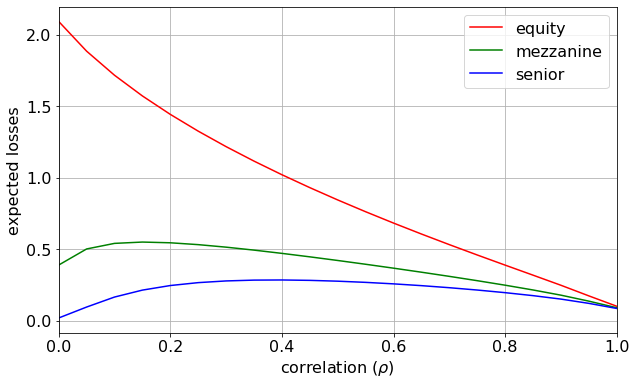
\includegraphics[width=0.7\textwidth]{figures/losses_vs_rho}
	\caption{Expected losses for each tranche as a function of the correlation parameter.}
	\label{fig:losses_rho}
\end{figure}

\begin{attention}
As noticed at the end of Section~\ref{standard-market-model}, in case the entities of the reference portfolio haven't the same default probabilities it is possible to determine Eq.~\ref{eq:def_prob_ex_cdo_1} numerically with an iterative procedure. The next snippet of code shows an example where ten names have different probabilities.

\begin{attpython}
N=10
# probabilities of default of the each name
q = [0.01, 0.02, 0.15, 0.22, 0.03, 0.01, 0.024, 0.008, 0.015, 0.04]

# p[k] probability of k defaults
p = [0 for _ in range(0, N+1)]
p[0] = (1-q[0])
p[1] = q[0]
for i in range(2, N+1):
    for j in range(1, i+1):
        p[j] = p[j-1]*q[i-1] + p[j]*(1-q[i-1])
    p[0] = p[0]*(1-q[i-1])
print (p)
\end{attpython}
\begin{ioutput}
[0.5655235318063276, 0.350403844356834, 0.11955743831716371,
 0.0330669128164737, 0.007898678014359, 0.00081191731818153,
 5.350491409986e-05, 2.81423807427e-06, 1.2554827537575e-07,
 5.216612301099e-09, 2.08664492043e-10]
\end{ioutput}
\end{attention}

\subsection{Synthetic CDO Valuation}
Imagine a Synthetic CDO made of $N$ references in the portfolio, each one with the same notional amount (the total CDO notional is $F$).
When the $i^{th}$ reference defaults the portfolio incurs in a loss of $\frac{F}{N}(1-R)$ (the recovery rate is assumed to be the same for all names).

The tranche loss function $TL^{L,U}(l)$ for a given time $t$ is a function of the number of defaults $l$ occurred up to that time and is given by
\begin{equation}
TL_{t}^{L,U}=\mathrm{max}(\mathrm{min}(\cfrac{l}{N}\cdot F(1-R), U)-L, 0)
\end{equation}
where $\frac{l}{N}F(1-R)$ is the total portfolio loss, if it is greater than $U$ then the tranche loss is $U$, conversely if it is lower than $L$ there is no loss.

So for example suppose $L=3\%$ and $U=7\%$ and suppose also that the portfolio loss is $5\%$. Then the tranche loss is 2\% of the total portfolio notional (or 50\% of the tranche notional $=7\%-3\%=4\%$).

When an investor \emph{sells protection} on a tranche she is guaranteeing to reimburse any realized losses on the tranche to the \emph{protection buyer} (to better understand this concept it is useful to think of the protection as an \emph{insurance}). 
In return, the protection seller receives a premium at regular intervals (typically every three months) from the protection buyer.

\subsubsection{Premium Leg}
The premium leg payments are made at the end of each time interval and are proportional to the \textbf{remaining notional} in the tranche (this is another important difference with respect to CDS, where the contract ends as soon as a default occurs).

We can then write the NPV of the premium leg as

\begin{equation}
\mathrm{NPV}_{\mathrm{premium}}^{L,U}=S\sum^{n}_{i=1}D(d_i)\cfrac{(d_i - d_{i-1})}{360}\left(F(U-L)-\mathbb{E}[TL_{d-1}^{L,U}]\right)
\label{eq:cdo_npv_premium}
\end{equation}
where $n$ is the number of payment dates, $D(d_i)$ is the discount factor, $S$ is the annualized premium. The expected value represents the tranche loss at time $d_{i-1}$. Note that for simplicity we are ignoring that the default may take place at any time between each payment date.

\subsubsection{Default Leg}
The default leg represents the cash flows paid to the protection buyer upon losses occurring in the considered tranche. 

The NPV of the leg can be expressed as
\begin{equation}
\mathrm{NPV}_{\mathrm{default}}^{L,U}=\sum_{i=1}^{n}D(d_i)\left(\mathbb{E}[TL_{d_i}^{L,U}]-\mathbb{E}[TL_{d_{i-1}}^{L,U}]\right)
\label{eq:cdo_npv_default}
\end{equation}
where the argument in parenthesis is the expected losses between time $d_{i-1}$ up to $d_i$. 

From Equations~\ref{eq:cdo_npv_premium} and~\ref{eq:cdo_npv_default} it is clear that the key ingredient for the valuation of a CDO is the calculation of $\mathbb{E}[TL_{d_i}^{L,U}]$ which appears in both. Luckily using the Gaussian copula it is relatively easy to compute it. Indeed we know that 
\begin{equation}
TL_{t}^{L,U}=\mathrm{max}(\mathrm{min}(\frac{l}{N}\cdot F(1-R), U)-L, 0)
\label{eq:tl}
\end{equation}
where the only random variable is the number of defaults $l$. We also know that 
\begin{equation}
\mathbb{E}[TL_{t}^{L,U}] = \sum_{l=0}^{N}TL_{t}^{L,U}\cdot \int_{-\infty}^{\infty} P_{\mathrm{def}}(l(t|M)=j) \phi(M)dM
\label{eq:etl}
\end{equation}

And has we have already seen this calculation can be carried on without too much effort. The large popularity of the Gaussian copula just resides in this, it allows to compute very quickly very complicated contracts like CDOs which usually involve a large number of correlated names.

\subsection{CDO Fair Value}
The \emph{fair value} of a CDO tranche is that value of the premium $S^*$ for which the expected value of the premium leg equals the expected value of the default leg and for what we have seen depends on the expected value of the tranche loss function.

Given Equations~\ref{eq:cdo_npv_premium} and~\ref{eq:cdo_npv_default} it can be expressed as

\begin{equation}
S^* = \cfrac{\mathrm{NPV_{default}}^{L,U}}{\sum^{n}_{i=1}D(d_i)\cfrac{(d_i - d_{i-1})}{360}\left(F(U-L)-\mathbb{E}[TL_{d-1}^{L,U}]\right)}
\label{eq:cdo_fair_value}
\end{equation}

Equation~\ref{eq:cdo_fair_value} defines the CDO fair value, but can also be used to calibrate the implied correlation parameter from the market. This can be obtained by plugging into the equation the market premium value and solve for the correlation parameter $\rho$. It must be noted though that the derivation of the implied correlation coefficient is not that easy since the assumed model is so simple that may not fit well to real data. Indeed it is most likely that there will be different implied $\rho$s for each tranche (while the model assumes the same correlation everywhere).

As a last consideration we have to notice that all equations shown previously have been derived under the assumptions of the same notional and recovery rate for each entity in the portfolio. Nonetheless their generalization to different notional and recovery rate is pretty straightforward.
 
%Each tranche has an attachment percentage and a detachment
%percentage. When the cumulative percentage loss of the portfolio reaches
%the attachment percentage, investors in the tranche start to lose their
%principal, and when the cumulative percentage loss of principal reaches
%the detachment percentage, the investors in the tranche lose all their
%principal and no further loss can occur to them.
%
%A common analogy compares the cash flow from the CDO's portfolio of securities (say mortgage payments from mortgage-backed bonds) to water flowing into cups of the investors where senior tranches were filled first and overflowing cash flowed to junior tranches, then equity tranches. If a large portion of the mortgages enter default, there is insufficient cash flow to fill all these cups and equity tranche investors face the losses first.

\begin{finmarkets}
Clearly this class too has to go into the \texttt{finmarkets} module. The following code implements a \texttt{CollDebtObligation} class.
\end{finmarkets}

\begin{ipython}
import numpy as np
from finmarkets import DiscountCurve, CreditCurve, generate_dates
from scipy.integrate import quad
from scipy.stats import norm, binom

class CollDebtObligation:
    def __init__(self, nominal, N, tranches, rho, cc,
                 start_date, spreads, maturity, tenor="3m", recovery=0.4):
        self.nominal = nominal
        self.N = N
        self.tranches = tranches
        self.payment_dates = generate_dates(start_date, maturity, tenor)
        self.spreads = spreads
        self.rho = rho
        self.recovery = recovery
        self.cc = cc

    def one_factor_model(self, M, Q, l, L, U):
        P = norm.cdf((norm.ppf(Q) - np.sqrt(self.rho) * M) / (np.sqrt(1 - self.rho)))
        b = binom(self.N, P)
        return b.pmf(l) * norm.pdf(M) * max(min(l/self.N *
               self.nominal * (1 - self.recovery), U) - L, 0)

    def expected_tranche_loss(self, d, L, U):
        Q = 1 - self.cc.ndp(d)
        v = 0 
        for l in range(self.N+1):
            i = quad(self.one_factor_model, -np.inf, np.inf,
                args=(Q, l, L, U))[0]
            v += i
        return v

    def npv_premium(self, tranche, dc):
        L = self.tranches[tranche][0] * self.nominal
        U = self.tranches[tranche][1] * self.nominal
        v = 0
        for i in range(1, len(self.payment_dates)):
            ds = self.payment_dates[i - 1]
            de = self.payment_dates[i]
            D = dc.df(de)
            ETL = self.expected_tranche_loss(ds, L, U)
            v += D * (de - ds).days / 360 * max((U - L) - ETL, 0)
        return v * self.spreads[tranche]

    def npv_default(self, tranche, dc):
        U = self.tranches[tranche][1] * self.nominal
        L = self.tranches[tranche][0] * self.nominal
        v = 0
        for i in range(1, len(self.payment_dates)):
            ds = self.payment_dates[i - 1]
            de = self.payment_dates[i]
            ETL1 = self.expected_tranche_loss(ds, L, U)
            ETL2 = self.expected_tranche_loss(de, L, U)
            v += dc.df(de) * (ETL2 - ETL1)
        return v

    def npv(self, tranche, dc):
        return self.npv_default(tranche, dc) - self.npv_premium(tranche, dc)

    def fair_value(self, tranche, dc):
        num = self.npv_default(tranche, dc)
        den = self.npv_premium(tranche, dc) / self.spreads[tranche]
        return num / den
\end{ipython}

Let's test the class with a CDO with 1 year maturity and a reference portfolio of 125 names. Each of them have the same default probabilities, defined through a credit curve (\texttt{cc}) and the correlation is set to 0.3. The risk free rate is flat at 5\%. The tenor has been chosen to 12 months mainly for performance reasons since the computation of the expected losses implies the integration in Equations~\ref{eq:tl} and \ref{eq:etl}, for each name, and for each payment date and this can be quite time consuming.
Tranches and premiums are defined as follows:
\begin{itemize}
	\item equity: [0.0, 0.03] (spread 0.15);
	\item mezzanine: [0.03, 0.06] (spread 0.07);
	\item senior: [0.06, 0.09] (spread 0.03);
	\item super-senior: [0.09, 1.0] (spread 0.01).
\end{itemize}

In the following example we are going to evaluate the fair value of each tranche of the contract.

\begin{ipython}
from finmarkets import DiscountCurve, CreditCurve
from datetime import date
from dateutil.relativedelta import relativedelta

pillar_dates = []
df = []
obs_date = date.today()
start_date = obs_date
for i in range(1, 2):
    pillar_dates.append(obs_date + relativedelta(years=i))
    df.append(1 / (1 + 0.05) ** i)
dc = DiscountCurve(obs_date, pillar_dates, df)
cc = CreditCurve(obs_date, 
                 [obs_date + relativedelta(years=i) for i in range(1, 5)],
                 [0.99, 0.97, 0.95, 0.93])
tranches = [[0.0, 0.03], [0.03, 0.06], [0.06, 0.09], [0.09, 1.0]]
spreads = [0.15, 0.07, 0.03, 0.01]
cdo = CollDebtObligation(100e6, 125, tranches, 0.3, cc,
                         start_date, spreads, "1y", "12m")
          
for i in range(len(tranches)):
    print (f"Tranche {i} ({tranches[i]}): {cdo.fair_value(i, dc):.5f}")
\end{ipython}
\begin{ioutput}
Tranche 0 ([0.0, 0.03]): 0.15942
Tranche 1 ([0.03, 0.06]): 0.02505
Tranche 2 ([0.06, 0.09]): 0.00773
Tranche 3 ([0.09, 1.0]): 0.00017
\end{ioutput}

As expected the equity tranche has the higher fair value being the riskier, while the senior tranche is the safest hence the one with lower premium.

\section*{Exercises}
\begin{question}
Six companies have default probabilities of 1\%, 2\%, 5\%, 8\%, 11\% respectively for each of the next five years. Also the probabilities are correlated by $\rho=0.4$. Determine the 4th-to-default probabilities for each year when a Gaussian copula is used to model the defaults.
\end{question}

\cprotEnv\begin{solution}

The covariance matrix of the multivariate normal distribution has bee constructed by starting with a matrix whose values are all equal to $\rho$, then the diagonal elements have been zeroed.

\begin{ipython}
from scipy.stats import multivariate_normal, norm

p_default = [0, 0.01, 0.02, 0.05, 0.08, 0.11]
cov = np.ones(shape=(6, 6))*0.4
np.fill_diagonal(cov, 1.0)
mvnorm = multivariate_normal(mean=[0]*6, cov=cov)

n_to_default = 4
trials = 500000
result = [0., 0., 0., 0., 0., 0.]
x = mvnorm.rvs(size=trials)
sim_defaults = np.sort(norm.cdf(x))

for s in sim_defaults:
    for i in range(1, len(p_default)):
        if p_default[i-1] <= s[n_to_default-1] <= p_default[i]:
            result[i] += 1

print ("4th-to-default probabilities")
for i in range(len(p_default)):
    print (f"{i}: {result[i]/trials:.4f}")
\end{ipython}
\begin{ioutput}
4th-to-default probabilities
0: 0.0000
1: 0.0004
2: 0.0009
3: 0.0059
4: 0.0098
5: 0.0135
\end{ioutput}
\end{solution}

\begin{question}
Consider a 3-year 5th-to-default basket on ten reference entities in the situation where the copula correlation is 0.15 and the expected recovery rate, $R$, is $40\%$. The term structure of interest rates is assumed to be flat at 3\%. The default probabilities for the entities are 1\%, 3\% and 7\% respectively in one, two and three years from now.
Determine the breakeven rate and the NPV of the contract.
\end{question}

\cprotEnv\begin{solution}	
\begin{ipython}
from finmarkets import DiscountCurve, BasketDefaultSwaps
from datetime import date
from dateutil.relativedelta import relativedelta

n_cds = 10
rho = 0.15
l = 0.016
ndefaults = 5

obs_date = date.today()
start_date = obs_date
dates = [obs_date + relativedelta(years=i) for i in range(1, 4)]
dfs = [1/(1+0.03)**i for i in range(1, 4)]
dc = DiscountCurve(obs_date, dates, dfs)

basket = BasketDefaultSwaps(1e6, n_cds, l, rho, start_date, "3y", 0.01)
basket.credit_curve(obs_date, dates, ndefaults)
bkeven = basket.breakeven(dc)
print(f"breakeven rate: {bkeven:.5f}:")

new_basket = BasketDefaultSwaps(1e6, n_cds, l, rho, start_date, "3y", bkeven)
new_basket.credit_curve(obs_date, dates, ndefaults)
print(f"NPV: {new_basket.npv(dc):.0f}")
\end{ipython}
\begin{ioutput}
breakeven: 0.00017
NPV: -263
\end{ioutput}
\end{solution}

\begin{question}
Consider a Cash CDO with a maturity of 1 year, made of 125 bonds. Each bond pays a coupon of one unit after 1 year and it has not yet defaulted (the recovery rate $R$ is assumed 0). The CDO has three tranches: equity ([0, 3] defaults), mezzanine ([4, 6] defaults) and senior ([7, 125] defaults).
Draw the expected loss as a function of the correlation $\rho$ for the three tranches and show that the sum of the losses of each tranche is independent from $\rho$.
\end{question}

\cprotEnv\begin{solution}	
To solve this question we need to implement a function that evaluate through the one-factor copula model and the binomial distribution the probability of $l$ defaults.
Then we can compute the expected losses for each tranche and for various values of the correlation parameter $\rho$, saving into a list the results for later plotting.

\begin{ipython}
from scipy.stats import binom, norm
from scipy.integrate import quad
import numpy as np

N = 125
A = 1
R = 0
M = 1
q = 0.02
tranches = [[1,3],[4, 6],[7,125]]
def p(M, rho, lims):
    qM = max(1e-10, norm.cdf((norm.ppf(q)-np.sqrt(rho)*M)/(np.sqrt(1-rho))))
    pN = binom(N, qM)
    prob = (lims[1]-lims[0]+1) * (pN.cdf(N) - pN.cdf(lims[1]-1))
    for i in range(lims[0], lims[1]):
        prob += (i-lims[0]+1)*pN.pmf(i)
    return norm.pdf(M)*prob

res = [[],[],[]]
for i in range(len(tranches)):
    for rho in np.arange(0., 1.05, 0.1):
        if rho == 1.0:
            rho = 0.99
        v = quad(p, -np.inf, np.inf, args=(rho, tranches[i]))
        res[i].append(v[0])
\end{ipython}

\begin{figure}[htbp]
\begin{center}		
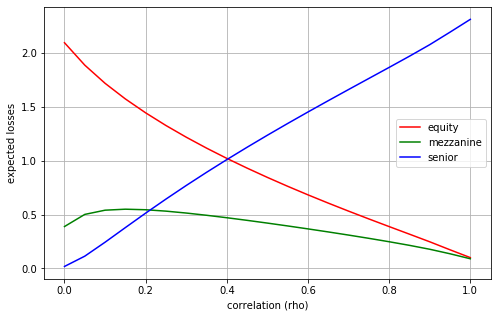
\includegraphics[width=0.7\linewidth]{figures/losses_vs_rho_2}
\end{center}
\end{figure}

To demonstrate that the total expected loss is independent from $\rho$ it is enough to print its values for a couple of different values of the correlation parameter. Since the expected loss of the tranches have been saved into lists the sum can be done among values of the lists with similar indices. 

\begin{ipython}
print (res[0][1] + res[1][1] + res[2][1])
print (res[0][5] + res[1][5] + res[2][5])
print (res[0][9] + res[1][9] + res[2][9])
\end{ipython}
\begin{ioutput}
2.500000000000001
2.5000000000019336
2.5000000062236856
\end{ioutput}
\end{solution}

\begin{question}
Determine the fair value of each tranche in a CDO with 1 year maturity and a reference portfolio of 125 names. Each of them have the same default probabilities, 1\%, and their correlation is set to 0.2. The tenor of the premium leg is 12 months. The risk free rate is flat at 5\%.
\begin{itemize}
	\item equity: [0.0, 0.03] (spread 0.20);
	\item mezzanine: [0.03, 0.06] (spread 0.01);
	\item senior: [0.06, 1.0] (spread 0.005).
\end{itemize}
How does these results change if the default probability raises to 5\% ? \\
How does these results change if instead there is an higher correlation (0.6) ?
\end{question}

\cprotEnv\begin{solution}

\begin{ipython}
from finmarkets import DiscountCurve, CreditCurve, CollDebtObligation
from datetime import date
from dateutil.relativedelta import relativedelta

pillar_dates = []
df = []
obs_date = date.today()
start_date = obs_date
dates = [obs_date + relativedelta(years=i) for i in range(1, 2)]
dfs = [1/(1 + 0.05)**i for i in range(1, 2)]
dc = DiscountCurve(obs_date, dates, dfs)

cc = CreditCurve(obs_date,
                 [obs_date + relativedelta(years=i) for i in range(1, 5)],
                 [0.99, 0.97, 0.95, 0.93])

nnames = 125
tranches = [[0.0, 0.03], [0.03, 0.06], [0.06, 0.09], [0.09, 1.0]]
spreads = [0.15, 0.07, 0.03, 0.01]

cdo = CollDebtObligation(100e6, nnames, tranches,
                         0.3, cc, start_date, spreads,
                         "1y", "12m")

for i in range(len(tranches)):
    print (f"Tranche {i} ({tranches[i]}): {cdo.fair_value(i, dc):.5f}")
\end{ipython}
\begin{ioutput}
Tranche 0 ([0.0, 0.03]): 0.17775
Tranche 1 ([0.03, 0.06]): 0.01570
Tranche 2 ([0.06, 1.0]): 0.00012
\end{ioutput}
With an higher default probability instead, the NPV of the default leg increases and so does the fair value.

\begin{ioutput}
Tranche 0 ([0.0, 0.03]): 0.59296
Tranche 1 ([0.03, 0.06]): 0.22714
Tranche 2 ([0.06, 1.0]): 0.00530
\end{ioutput}
Finally with a larger correlation the probability of multiple defaults increases leading to larger losses in safer tranches. So the fair value increases in mezzanine and senior tranches, but is lower in the equity where the probability of few defaults is reduced.

\begin{ioutput}
Tranche 0 ([0.0, 0.03]): 0.09899
Tranche 1 ([0.03, 0.06]): 0.03498
Tranche 2 ([0.06, 1.0]): 0.00192
\end{ioutput}
\end{solution}


\begin{thebibliography}{9}
\bibitem{bib:cdo} J. C. Hull, \emph{Options, Futures and Other Derivatives, 7th Ed.}, Credit Derivatives (Ch. 23), Pearson Prentice Hall, 2009
\bibitem{bib:bds} J. C. Hull, A. White, \href{http://www-2.rotman.utoronto.ca/~hull/downloadablepublications/HullWhiteCDOPaper.pdf}{\emph{Valuation of a CDO and an nth to Default CDS Without Monte Carlo Simulation}}, Journal of Derivatives, 12,2, Winter 2004,  Online 
\end{thebibliography}
